\section{Устойчивость равновесия консервативных систем}

Пусть $q = 0$ -- положения равновесия. Динамика нашей системы описывается уравнениями Лагранжа, вида
\begin{equation*}
    \frac{d }{d t} \frac{\partial L}{\partial \dot{q}} - \frac{\partial L}{\partial q} = 0.
\end{equation*}
Также говорим про консервативную систему, то есть все связи склерономны,
\begin{equation*}
    \exists \Pi \equiv \Pi (q); \hspace{0.5cm} 
    f(t, \vc{r}) = 0 \hspace{0.5cm} \Rightarrow \hspace{0.5cm} 
    T + \Pi = \const.
\end{equation*}
\begin{to_def} 
    Положение равновесия $q=0$ -- \textit{устойчиво по Ляпунову}, если $\forall \varepsilon > 0 \ \exists \delta > 0$, такая что 
\begin{equation}
    \forall |q(0)|<\delta, \ |\dot{q}(0)|<\delta \colon
    \hspace{0.5cm} 
    |q(t)|<\varepsilon, \ |\dot{q}(t)| < \varepsilon, \hspace{0.5cm} \forall t \geq 0.
\end{equation}
\end{to_def}

\begin{to_def} 
    Положение равновесия $q=0$ -- \textit{неустойчиво по Ляпунову}, если $\exists \varepsilon > 0 \ \forall \delta > 0$, такая что 
\begin{equation}
    \forall \delta > 0 \ \exists |q(0)| < \delta, 
    |\dot{q}(0)| < \delta, t^* \colon \hspace{0.5cm} 
    |q(t^*)| > \varepsilon \text{ или } |\dot{q}(t^*)| > \varepsilon.
\end{equation}
\end{to_def}

\begin{to_thr}[Теорема Лагранжа-Дирихле]
     Если в положении равновесия $\Pi(q)$ имеет строгий локальный минимум, то это положение равновесия устойчиво.
\end{to_thr}

\noindent
Разложим в ряд $\Pi(q)$:
\begin{equation*}
    \Pi (q) = 
    {\Pi (0)}
     + 
     {\frac{\partial \Pi}{\partial q^i} \bigg|_0 q^i }+ \frac{1}{2} \frac{\partial^2 \Pi}{\partial q^i \partial q^k} + \ldots
     \approx \frac{1}{2} \frac{\partial^2 \Pi}{\partial q^i \partial q^k}.
\end{equation*}

\begin{to_thr}[Теорма Ляпунова о неустойчивости I]
    Если в положении равновесия $\Pi(q)$ не имеет минимума и это определяется по квадратичной форме её разложения в ряд (в окрестности положения равновесия), то это положение равновесия неустойчиво.     
\end{to_thr}


\begin{to_thr}[Теорма Ляпунова о неустойчивости II]
    Если в положении равновесия $\Pi(q)$  имеет строгий максимум и это определяется по наинизшей степени её разложения в ряд (в окрестности положения равновесия), то это положение равновесия неустойчиво.     
\end{to_thr}


\subsection*{Задача 1 (15.6)}

\begin{equation*}
    \Pi = mgl (1 - \cos \varphi) - m \omega^2 (l^2 \sin^2 \varphi) / 2.
\end{equation*}

Найдём положения равновесия, как стационарные точки потенциала
\begin{equation*}
    \frac{d \Pi}{d \varphi} = mgl \sin \varphi - m \omega^2 l^2 \sin \varphi \cos \varphi = 0,
    \hspace{0.5cm} \Rightarrow \hspace{0.5cm} 
    \left\{\begin{aligned}
        \sin \varphi &= 0, \ &\varphi = 0 \pm \pi \\
        \cos \varphi &= g / \omega^2 l , \ 
        &\varphi = \pm \arccos g / \omega^2 l
    \end{aligned}\right.,
    \ \ \ \omega > \omega^* = \sqrt{\frac{g}{l} }
\end{equation*}
Посмотрим на
\begin{equation*}
    \frac{d^2 \Pi}{d \varphi^2} = 
    m l^2 \omega^2 \left(
        \frac{g}{\omega^2 l}  - 1
    \right)
\end{equation*}

При $\varphi = 0$, при $\omega < \omega^*$ видим устойчивое положение равновесия. При $\omega > \omega^*$ неустойчиво. 
При $\omega = \omega^*$ видимо, что
\begin{equation*}
    \frac{d^4 \Pi}{d \varphi^4} = ml^2 \omega^2 (-1 + 4) > 0
    \hspace{0.5cm} \Rightarrow \hspace{0.5cm} 
    \varphi = 0 \text{\ -- \ устойчиво}.
\end{equation*}

Теперь посмотрим на $\varphi = \pm \pi$:
\begin{equation*}
    \frac{d^2 \Pi}{d \varphi^2} < 0.
\end{equation*}

При $\cos \varphi = g / \omega^2 l$ видим, что
\begin{equation*}
    \frac{d^2 \Pi}{d \varphi^2} =
    ml^2 \omega^2 \left(
        \frac{g^2}{\omega^4 l^2}  + 1 
        - 2 \frac{g^2}{\omega^4 l^2} 
    \right) = 
    ml^2 \omega^2 \left(
        1 - \frac{g^2}{\omega^4 l^2} 
    \right),
\end{equation*}
видим, что $\omega > \omega^*$ положение равновесия устойчиво, при $\omega < \omega^*$ его попросту  не существует.

\begin{figure}[h]
    \centering
    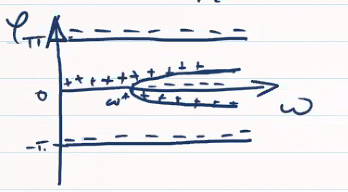
\includegraphics[width=0.25\textwidth]{figures/2.png}
    \caption{Бифуркационная диаграмма типа вилка}
\end{figure}


\subsection*{Задача 4 (Гандтмахер, устойчивость)}


\begin{equation*}
    \Pi = q^4 \sin^2 \frac{1}{q}, \hspace{0.5cm} \Pi(0) = 0, \hspace{0.5cm} q = 0 \text{\ -- п.р.}.
\end{equation*}

 